\batchmode
\documentclass[twoside]{book}

% Packages required by doxygen
\usepackage{fixltx2e}
\usepackage{calc}
\usepackage{doxygen}
\usepackage[export]{adjustbox} % also loads graphicx
\usepackage{graphicx}
\usepackage[utf8]{inputenc}
\usepackage{makeidx}
\usepackage{multicol}
\usepackage{multirow}
\PassOptionsToPackage{warn}{textcomp}
\usepackage{textcomp}
\usepackage[nointegrals]{wasysym}
\usepackage[table]{xcolor}

% Font selection
\usepackage[T1]{fontenc}
\usepackage[scaled=.90]{helvet}
\usepackage{courier}
\usepackage{amssymb}
\usepackage{sectsty}
\renewcommand{\familydefault}{\sfdefault}
\allsectionsfont{%
  \fontseries{bc}\selectfont%
  \color{darkgray}%
}
\renewcommand{\DoxyLabelFont}{%
  \fontseries{bc}\selectfont%
  \color{darkgray}%
}
\newcommand{\+}{\discretionary{\mbox{\scriptsize$\hookleftarrow$}}{}{}}

% Page & text layout
\usepackage{geometry}
\geometry{%
  a4paper,%
  top=2.5cm,%
  bottom=2.5cm,%
  left=2.5cm,%
  right=2.5cm%
}
\tolerance=750
\hfuzz=15pt
\hbadness=750
\setlength{\emergencystretch}{15pt}
\setlength{\parindent}{0cm}
\setlength{\parskip}{3ex plus 2ex minus 2ex}
\makeatletter
\renewcommand{\paragraph}{%
  \@startsection{paragraph}{4}{0ex}{-1.0ex}{1.0ex}{%
    \normalfont\normalsize\bfseries\SS@parafont%
  }%
}
\renewcommand{\subparagraph}{%
  \@startsection{subparagraph}{5}{0ex}{-1.0ex}{1.0ex}{%
    \normalfont\normalsize\bfseries\SS@subparafont%
  }%
}
\makeatother

% Headers & footers
\usepackage{fancyhdr}
\pagestyle{fancyplain}
\fancyhead[LE]{\fancyplain{}{\bfseries\thepage}}
\fancyhead[CE]{\fancyplain{}{}}
\fancyhead[RE]{\fancyplain{}{\bfseries\leftmark}}
\fancyhead[LO]{\fancyplain{}{\bfseries\rightmark}}
\fancyhead[CO]{\fancyplain{}{}}
\fancyhead[RO]{\fancyplain{}{\bfseries\thepage}}
\fancyfoot[LE]{\fancyplain{}{}}
\fancyfoot[CE]{\fancyplain{}{}}
\fancyfoot[RE]{\fancyplain{}{\bfseries\scriptsize Generated by Doxygen }}
\fancyfoot[LO]{\fancyplain{}{\bfseries\scriptsize Generated by Doxygen }}
\fancyfoot[CO]{\fancyplain{}{}}
\fancyfoot[RO]{\fancyplain{}{}}
\renewcommand{\footrulewidth}{0.4pt}
\renewcommand{\chaptermark}[1]{%
  \markboth{#1}{}%
}
\renewcommand{\sectionmark}[1]{%
  \markright{\thesection\ #1}%
}

% Indices & bibliography
\usepackage{natbib}
\usepackage[titles]{tocloft}
\setcounter{tocdepth}{3}
\setcounter{secnumdepth}{5}
\makeindex

% Hyperlinks (required, but should be loaded last)
\usepackage{ifpdf}
\ifpdf
  \usepackage[pdftex,pagebackref=true]{hyperref}
\else
  \usepackage[ps2pdf,pagebackref=true]{hyperref}
\fi
\hypersetup{%
  colorlinks=true,%
  linkcolor=blue,%
  citecolor=blue,%
  unicode%
}

% Custom commands
\newcommand{\clearemptydoublepage}{%
  \newpage{\pagestyle{empty}\cleardoublepage}%
}

\usepackage{caption}
\captionsetup{labelsep=space,justification=centering,font={bf},singlelinecheck=off,skip=4pt,position=top}

%===== C O N T E N T S =====

\begin{document}

% Titlepage & ToC
\hypersetup{pageanchor=false,
             bookmarksnumbered=true
            }
\pagenumbering{alph}
\pagenumbering{arabic}
\hypersetup{pageanchor=true}

%--- Begin generated contents ---
\chapter{Demo problem\+: Large-\/amplitude shock-\/wave propagation in a circular disk}
\label{index}\hypertarget{index}{}\hypertarget{index_q}{}\section{A few quick questions...}\label{index_q}
Since {\ttfamily oomph-\/lib} is developed as open-\/source software, any evidence that the code is being downloaded and used is very helpful for us as it helps to justify our continued work on this project.

We would therefore be extremely grateful if you could provide the information requested in the form below. Pressing the \char`\"{}submit\char`\"{} button will get you to the actual download page.

{\bfseries Note\+:} 
\begin{DoxyItemize}
\item All information will be treated as confidential. 
\item If you provide your email address and check the appropriate box we will add you to our mailing list to inform you of upgrades and bug fixes to the code. Rest assured that the mailing list is {\bfseries very low volume} -- we have better things to do than to bombard you with email. 
\item If you still feel reluctant to provide any of the information requested, feel free to enter some dummy input. The form will check that {\bfseries some} information has been entered but entering your name as \char`\"{}\+Joe Cool\char`\"{} is perfectly acceptable -- this is to discourage people from not providing the information simply because they are too lazy to type... 
\end{DoxyItemize}



 







 

 \hypertarget{index_pdf}{}\section{P\+D\+F file}\label{index_pdf}
A \href{../latex/refman.pdf}{\tt pdf version} of this document is available. \end{document}

\chapter{Namespace Index}
\section{Namespace List}
Here is a list of all namespaces with brief descriptions\+:\begin{DoxyCompactList}
\item\contentsline{section}{\hyperlink{namespaceGlobal__Physical__Variables}{Global\+\_\+\+Physical\+\_\+\+Variables} \\*Global variables that represent physical properties }{\pageref{namespaceGlobal__Physical__Variables}}{}
\item\contentsline{section}{\hyperlink{namespaceoomph}{oomph} }{\pageref{namespaceoomph}}{}
\item\contentsline{section}{\hyperlink{namespacePhysical__Variables}{Physical\+\_\+\+Variables} \\*Namespace for the solution of 2D linear shell equation }{\pageref{namespacePhysical__Variables}}{}
\end{DoxyCompactList}

\chapter{Hierarchical Index}
\section{Class Hierarchy}
This inheritance list is sorted roughly, but not completely, alphabetically\+:\begin{DoxyCompactList}
\item Problem\begin{DoxyCompactList}
\item \contentsline{section}{Unstructured\+Solid\+Problem$<$ E\+L\+E\+M\+E\+NT $>$}{\pageref{classUnstructuredSolidProblem}}{}
\end{DoxyCompactList}
\end{DoxyCompactList}

\chapter{Class Index}
\section{Class List}
Here are the classes, structs, unions and interfaces with brief descriptions\+:\begin{DoxyCompactList}
\item\contentsline{section}{\hyperlink{classPMLProblem}{P\+M\+L\+Problem$<$ E\+L\+E\+M\+E\+N\+T $>$} }{\pageref{classPMLProblem}}{}
\item\contentsline{section}{\hyperlink{classGlobalParameters_1_1TestPMLMapping}{Global\+Parameters\+::\+Test\+P\+M\+L\+Mapping} }{\pageref{classGlobalParameters_1_1TestPMLMapping}}{}
\end{DoxyCompactList}

\chapter{File Index}
\section{File List}
Here is a list of all files with brief descriptions\+:\begin{DoxyCompactList}
\item\contentsline{section}{\hyperlink{jeffery__orbit_8cc}{jeffery\+\_\+orbit.\+cc} }{\pageref{jeffery__orbit_8cc}}{}
\item\contentsline{section}{\hyperlink{jeffery__orbit_8txt__doxygenified_8h}{jeffery\+\_\+orbit.\+txt\+\_\+doxygenified.\+h} }{\pageref{jeffery__orbit_8txt__doxygenified_8h}}{}
\item\contentsline{section}{\hyperlink{my__taylor__hood__elements_8h}{my\+\_\+taylor\+\_\+hood\+\_\+elements.\+h} }{\pageref{my__taylor__hood__elements_8h}}{}
\end{DoxyCompactList}

\chapter{Namespace Documentation}
\hypertarget{namespaceGlobal__Physical__Variables}{}\section{Global\+\_\+\+Physical\+\_\+\+Variables Namespace Reference}
\label{namespaceGlobal__Physical__Variables}\index{Global\+\_\+\+Physical\+\_\+\+Variables@{Global\+\_\+\+Physical\+\_\+\+Variables}}


Namespace for physical parameters.  


\subsection*{Functions}
\begin{DoxyCompactItemize}
\item 
Vector$<$ double $>$ \hyperlink{namespaceGlobal__Physical__Variables_afae321364975eb56688ad13abc8ed6b7}{Gravity} (2)
\begin{DoxyCompactList}\small\item\em Gravity vector. \end{DoxyCompactList}\item 
void \hyperlink{namespaceGlobal__Physical__Variables_a87da705b8a46bed337cf5dbdd788b87b}{body\+\_\+force} (const double \&time, const Vector$<$ double $>$ \&x, Vector$<$ double $>$ \&result)
\begin{DoxyCompactList}\small\item\em Functional body force. \end{DoxyCompactList}\item 
void \hyperlink{namespaceGlobal__Physical__Variables_a9780d615ae07c4e00a436ab2973b54e6}{zero\+\_\+body\+\_\+force} (const double \&time, const Vector$<$ double $>$ \&x, Vector$<$ double $>$ \&result)
\begin{DoxyCompactList}\small\item\em Zero functional body force. \end{DoxyCompactList}\end{DoxyCompactItemize}
\subsection*{Variables}
\begin{DoxyCompactItemize}
\item 
double \hyperlink{namespaceGlobal__Physical__Variables_ab814e627d2eb5bc50318879d19ab16b9}{Re} =100
\begin{DoxyCompactList}\small\item\em Reynolds number. \end{DoxyCompactList}\item 
double \hyperlink{namespaceGlobal__Physical__Variables_ab1a845a672b4d74b304639a976dc65c6}{Re\+\_\+inv\+Fr} =100
\begin{DoxyCompactList}\small\item\em Reynolds/\+Froude number. \end{DoxyCompactList}\end{DoxyCompactItemize}


\subsection{Detailed Description}
Namespace for physical parameters. 

\subsection{Function Documentation}
\mbox{\Hypertarget{namespaceGlobal__Physical__Variables_a87da705b8a46bed337cf5dbdd788b87b}\label{namespaceGlobal__Physical__Variables_a87da705b8a46bed337cf5dbdd788b87b}} 
\index{Global\+\_\+\+Physical\+\_\+\+Variables@{Global\+\_\+\+Physical\+\_\+\+Variables}!body\+\_\+force@{body\+\_\+force}}
\index{body\+\_\+force@{body\+\_\+force}!Global\+\_\+\+Physical\+\_\+\+Variables@{Global\+\_\+\+Physical\+\_\+\+Variables}}
\subsubsection{\texorpdfstring{body\+\_\+force()}{body\_force()}}
{\footnotesize\ttfamily void Global\+\_\+\+Physical\+\_\+\+Variables\+::body\+\_\+force (\begin{DoxyParamCaption}\item[{const double \&}]{time,  }\item[{const Vector$<$ double $>$ \&}]{x,  }\item[{Vector$<$ double $>$ \&}]{result }\end{DoxyParamCaption})}



Functional body force. 



Definition at line 62 of file circular\+\_\+driven\+\_\+cavity.\+cc.



References Re\+\_\+inv\+Fr.



Referenced by main().

\mbox{\Hypertarget{namespaceGlobal__Physical__Variables_afae321364975eb56688ad13abc8ed6b7}\label{namespaceGlobal__Physical__Variables_afae321364975eb56688ad13abc8ed6b7}} 
\index{Global\+\_\+\+Physical\+\_\+\+Variables@{Global\+\_\+\+Physical\+\_\+\+Variables}!Gravity@{Gravity}}
\index{Gravity@{Gravity}!Global\+\_\+\+Physical\+\_\+\+Variables@{Global\+\_\+\+Physical\+\_\+\+Variables}}
\subsubsection{\texorpdfstring{Gravity()}{Gravity()}}
{\footnotesize\ttfamily Vector$<$double$>$ Global\+\_\+\+Physical\+\_\+\+Variables\+::\+Gravity (\begin{DoxyParamCaption}\item[{2}]{ }\end{DoxyParamCaption})}



Gravity vector. 



Referenced by main(), and Quarter\+Circle\+Driven\+Cavity\+Problem$<$ E\+L\+E\+M\+E\+N\+T $>$\+::\+Quarter\+Circle\+Driven\+Cavity\+Problem().

\mbox{\Hypertarget{namespaceGlobal__Physical__Variables_a9780d615ae07c4e00a436ab2973b54e6}\label{namespaceGlobal__Physical__Variables_a9780d615ae07c4e00a436ab2973b54e6}} 
\index{Global\+\_\+\+Physical\+\_\+\+Variables@{Global\+\_\+\+Physical\+\_\+\+Variables}!zero\+\_\+body\+\_\+force@{zero\+\_\+body\+\_\+force}}
\index{zero\+\_\+body\+\_\+force@{zero\+\_\+body\+\_\+force}!Global\+\_\+\+Physical\+\_\+\+Variables@{Global\+\_\+\+Physical\+\_\+\+Variables}}
\subsubsection{\texorpdfstring{zero\+\_\+body\+\_\+force()}{zero\_body\_force()}}
{\footnotesize\ttfamily void Global\+\_\+\+Physical\+\_\+\+Variables\+::zero\+\_\+body\+\_\+force (\begin{DoxyParamCaption}\item[{const double \&}]{time,  }\item[{const Vector$<$ double $>$ \&}]{x,  }\item[{Vector$<$ double $>$ \&}]{result }\end{DoxyParamCaption})}



Zero functional body force. 



Definition at line 70 of file circular\+\_\+driven\+\_\+cavity.\+cc.



Referenced by main().



\subsection{Variable Documentation}
\mbox{\Hypertarget{namespaceGlobal__Physical__Variables_ab814e627d2eb5bc50318879d19ab16b9}\label{namespaceGlobal__Physical__Variables_ab814e627d2eb5bc50318879d19ab16b9}} 
\index{Global\+\_\+\+Physical\+\_\+\+Variables@{Global\+\_\+\+Physical\+\_\+\+Variables}!Re@{Re}}
\index{Re@{Re}!Global\+\_\+\+Physical\+\_\+\+Variables@{Global\+\_\+\+Physical\+\_\+\+Variables}}
\subsubsection{\texorpdfstring{Re}{Re}}
{\footnotesize\ttfamily double Global\+\_\+\+Physical\+\_\+\+Variables\+::\+Re =100}



Reynolds number. 



Definition at line 53 of file circular\+\_\+driven\+\_\+cavity.\+cc.



Referenced by Quarter\+Circle\+Driven\+Cavity\+Problem$<$ E\+L\+E\+M\+E\+N\+T $>$\+::\+Quarter\+Circle\+Driven\+Cavity\+Problem().

\mbox{\Hypertarget{namespaceGlobal__Physical__Variables_ab1a845a672b4d74b304639a976dc65c6}\label{namespaceGlobal__Physical__Variables_ab1a845a672b4d74b304639a976dc65c6}} 
\index{Global\+\_\+\+Physical\+\_\+\+Variables@{Global\+\_\+\+Physical\+\_\+\+Variables}!Re\+\_\+inv\+Fr@{Re\+\_\+inv\+Fr}}
\index{Re\+\_\+inv\+Fr@{Re\+\_\+inv\+Fr}!Global\+\_\+\+Physical\+\_\+\+Variables@{Global\+\_\+\+Physical\+\_\+\+Variables}}
\subsubsection{\texorpdfstring{Re\+\_\+inv\+Fr}{Re\_invFr}}
{\footnotesize\ttfamily double Global\+\_\+\+Physical\+\_\+\+Variables\+::\+Re\+\_\+inv\+Fr =100}



Reynolds/\+Froude number. 



Definition at line 56 of file circular\+\_\+driven\+\_\+cavity.\+cc.



Referenced by body\+\_\+force(), and Quarter\+Circle\+Driven\+Cavity\+Problem$<$ E\+L\+E\+M\+E\+N\+T $>$\+::\+Quarter\+Circle\+Driven\+Cavity\+Problem().


\chapter{Class Documentation}
\hypertarget{classDiskShockWaveProblem}{}\section{Disk\+Shock\+Wave\+Problem$<$ E\+L\+E\+M\+E\+NT, T\+I\+M\+E\+S\+T\+E\+P\+P\+ER $>$ Class Template Reference}
\label{classDiskShockWaveProblem}\index{Disk\+Shock\+Wave\+Problem$<$ E\+L\+E\+M\+E\+N\+T, T\+I\+M\+E\+S\+T\+E\+P\+P\+E\+R $>$@{Disk\+Shock\+Wave\+Problem$<$ E\+L\+E\+M\+E\+N\+T, T\+I\+M\+E\+S\+T\+E\+P\+P\+E\+R $>$}}
Inheritance diagram for Disk\+Shock\+Wave\+Problem$<$ E\+L\+E\+M\+E\+NT, T\+I\+M\+E\+S\+T\+E\+P\+P\+ER $>$\+:\begin{figure}[H]
\begin{center}
\leavevmode
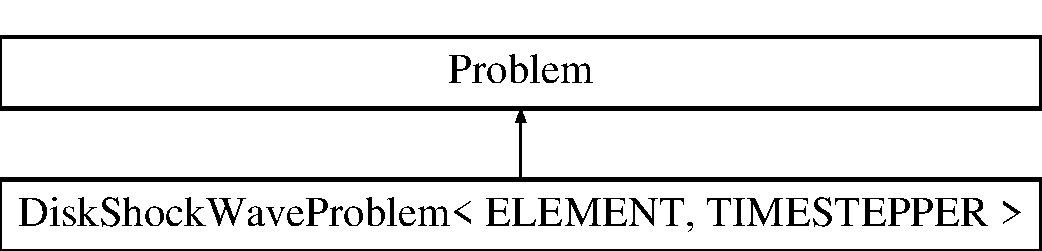
\includegraphics[height=2.000000cm]{classDiskShockWaveProblem}
\end{center}
\end{figure}
\subsection*{Public Member Functions}
\begin{DoxyCompactItemize}
\item 
\hyperlink{classDiskShockWaveProblem_ae670d0120936f410134ba3e3b61aa880}{Disk\+Shock\+Wave\+Problem} ()
\begin{DoxyCompactList}\small\item\em Constructor\+: \end{DoxyCompactList}\item 
void \hyperlink{classDiskShockWaveProblem_af8dc3befd3eba59b008c315bfe077340}{run} (const unsigned \&case\+\_\+number)
\begin{DoxyCompactList}\small\item\em Run the problem; specify case\+\_\+number to label output directory. \end{DoxyCompactList}\item 
\hyperlink{classElasticRefineableQuarterCircleSectorMesh}{Elastic\+Refineable\+Quarter\+Circle\+Sector\+Mesh}$<$ E\+L\+E\+M\+E\+NT $>$ $\ast$\& \hyperlink{classDiskShockWaveProblem_a558dc0ca72e4e1974c98cdf5203d015b}{solid\+\_\+mesh\+\_\+pt} ()
\begin{DoxyCompactList}\small\item\em Access function for the solid mesh. \end{DoxyCompactList}\item 
Solid\+Mesh $\ast$\& \hyperlink{classDiskShockWaveProblem_aade14ed9df7e698c3e90abea96090ab5}{traction\+\_\+mesh\+\_\+pt} ()
\begin{DoxyCompactList}\small\item\em Access function for the mesh of surface traction elements. \end{DoxyCompactList}\item 
void \hyperlink{classDiskShockWaveProblem_a7685309caac199d18f3f81468d9fcb23}{doc\+\_\+solution} ()
\begin{DoxyCompactList}\small\item\em Doc the solution. \end{DoxyCompactList}\item 
void \hyperlink{classDiskShockWaveProblem_a46f6a25da58128f6abfdbbe92ea49d11}{actions\+\_\+after\+\_\+newton\+\_\+solve} ()
\begin{DoxyCompactList}\small\item\em Update function (empty) \end{DoxyCompactList}\item 
void \hyperlink{classDiskShockWaveProblem_a50ba8e9b29ff7796fa9cb7ede8598376}{actions\+\_\+before\+\_\+newton\+\_\+solve} ()
\begin{DoxyCompactList}\small\item\em Update function (empty) \end{DoxyCompactList}\item 
void \hyperlink{classDiskShockWaveProblem_ac2a22a8399355e461d1a9ad1e5425c9a}{actions\+\_\+after\+\_\+adapt} ()
\begin{DoxyCompactList}\small\item\em Actions after adaption\+: Kill and then re-\/build the traction elements on boundary 1 and re-\/assign the equation numbers. \end{DoxyCompactList}\item 
void \hyperlink{classDiskShockWaveProblem_a75403423b0a031adabb5b487fa88373f}{doc\+\_\+displ\+\_\+and\+\_\+veloc} (const int \&stage=0)
\begin{DoxyCompactList}\small\item\em Doc displacement and velocity\+: label file with before and after. \end{DoxyCompactList}\item 
void \hyperlink{classDiskShockWaveProblem_a2eaf91d3e0eb5f37b9920fc3d9d54cb9}{dump\+\_\+it} (ofstream \&dump\+\_\+file)
\begin{DoxyCompactList}\small\item\em Dump problem-\/specific parameters values, then dump generic problem data. \end{DoxyCompactList}\item 
void \hyperlink{classDiskShockWaveProblem_ae883625e9bbe6ea442413f7c970d3fb1}{restart} (ifstream \&restart\+\_\+file)
\begin{DoxyCompactList}\small\item\em Read problem-\/specific parameter values, then recover generic problem data. \end{DoxyCompactList}\end{DoxyCompactItemize}
\subsection*{Private Attributes}
\begin{DoxyCompactItemize}
\item 
Doc\+Info \hyperlink{classDiskShockWaveProblem_a8e445e31a1067ebbd3bd667cc02e8662}{Doc\+\_\+info}
\item 
ofstream \hyperlink{classDiskShockWaveProblem_a8ec35b07dc6870e4d5b729288053c4fe}{Trace\+\_\+file}
\begin{DoxyCompactList}\small\item\em Trace file. \end{DoxyCompactList}\item 
Vector$<$ Node $\ast$ $>$ \hyperlink{classDiskShockWaveProblem_a7ab6db65bbf28185b238e84bbc16c1b8}{Trace\+\_\+node\+\_\+pt}
\begin{DoxyCompactList}\small\item\em Vector of pointers to nodes whose position we\textquotesingle{}re tracing. \end{DoxyCompactList}\item 
\hyperlink{classElasticRefineableQuarterCircleSectorMesh}{Elastic\+Refineable\+Quarter\+Circle\+Sector\+Mesh}$<$ E\+L\+E\+M\+E\+NT $>$ $\ast$ \hyperlink{classDiskShockWaveProblem_a6efbcb695e829d63f810a7a9bb5a81a4}{Solid\+\_\+mesh\+\_\+pt}
\begin{DoxyCompactList}\small\item\em Pointer to solid mesh. \end{DoxyCompactList}\item 
Solid\+Mesh $\ast$ \hyperlink{classDiskShockWaveProblem_a286fe7d51aa16f07f0444ae7c553f140}{Traction\+\_\+mesh\+\_\+pt}
\begin{DoxyCompactList}\small\item\em Pointer to mesh of traction elements. \end{DoxyCompactList}\end{DoxyCompactItemize}


\subsection{Detailed Description}
\subsubsection*{template$<$class E\+L\+E\+M\+E\+NT, class T\+I\+M\+E\+S\+T\+E\+P\+P\+ER$>$\newline
class Disk\+Shock\+Wave\+Problem$<$ E\+L\+E\+M\+E\+N\+T, T\+I\+M\+E\+S\+T\+E\+P\+P\+E\+R $>$}

\char`\"{}\+Shock\char`\"{} wave propagates through an impulsively loaded circular disk. 

Definition at line 211 of file shock\+\_\+disk.\+cc.



\subsection{Constructor \& Destructor Documentation}
\mbox{\Hypertarget{classDiskShockWaveProblem_ae670d0120936f410134ba3e3b61aa880}\label{classDiskShockWaveProblem_ae670d0120936f410134ba3e3b61aa880}} 
\index{Disk\+Shock\+Wave\+Problem@{Disk\+Shock\+Wave\+Problem}!Disk\+Shock\+Wave\+Problem@{Disk\+Shock\+Wave\+Problem}}
\index{Disk\+Shock\+Wave\+Problem@{Disk\+Shock\+Wave\+Problem}!Disk\+Shock\+Wave\+Problem@{Disk\+Shock\+Wave\+Problem}}
\subsubsection{\texorpdfstring{Disk\+Shock\+Wave\+Problem()}{DiskShockWaveProblem()}}
{\footnotesize\ttfamily template$<$class E\+L\+E\+M\+E\+NT , class T\+I\+M\+E\+S\+T\+E\+P\+P\+ER $>$ \\
\hyperlink{classDiskShockWaveProblem}{Disk\+Shock\+Wave\+Problem}$<$ E\+L\+E\+M\+E\+NT, T\+I\+M\+E\+S\+T\+E\+P\+P\+ER $>$\+::\hyperlink{classDiskShockWaveProblem}{Disk\+Shock\+Wave\+Problem} (\begin{DoxyParamCaption}{ }\end{DoxyParamCaption})}



Constructor\+: 

Constructor. 

Definition at line 286 of file shock\+\_\+disk.\+cc.



References Global\+\_\+\+Physical\+\_\+\+Variables\+::constant\+\_\+pressure(), Global\+\_\+\+Physical\+\_\+\+Variables\+::\+Constitutive\+\_\+law\+\_\+pt, and Elastic\+Refineable\+Quarter\+Circle\+Sector\+Mesh$<$ E\+L\+E\+M\+E\+N\+T $>$\+::make\+\_\+traction\+\_\+element\+\_\+mesh().



\subsection{Member Function Documentation}
\mbox{\Hypertarget{classDiskShockWaveProblem_ac2a22a8399355e461d1a9ad1e5425c9a}\label{classDiskShockWaveProblem_ac2a22a8399355e461d1a9ad1e5425c9a}} 
\index{Disk\+Shock\+Wave\+Problem@{Disk\+Shock\+Wave\+Problem}!actions\+\_\+after\+\_\+adapt@{actions\+\_\+after\+\_\+adapt}}
\index{actions\+\_\+after\+\_\+adapt@{actions\+\_\+after\+\_\+adapt}!Disk\+Shock\+Wave\+Problem@{Disk\+Shock\+Wave\+Problem}}
\subsubsection{\texorpdfstring{actions\+\_\+after\+\_\+adapt()}{actions\_after\_adapt()}}
{\footnotesize\ttfamily template$<$class E\+L\+E\+M\+E\+NT , class T\+I\+M\+E\+S\+T\+E\+P\+P\+ER $>$ \\
void \hyperlink{classDiskShockWaveProblem}{Disk\+Shock\+Wave\+Problem}$<$ E\+L\+E\+M\+E\+NT, T\+I\+M\+E\+S\+T\+E\+P\+P\+ER $>$\+::actions\+\_\+after\+\_\+adapt (\begin{DoxyParamCaption}{ }\end{DoxyParamCaption})}



Actions after adaption\+: Kill and then re-\/build the traction elements on boundary 1 and re-\/assign the equation numbers. 

Kill and then re-\/build the traction elements on boundary 1, pin redundant pressure dofs and re-\/assign the equation numbers. 

Definition at line 440 of file shock\+\_\+disk.\+cc.



References Global\+\_\+\+Physical\+\_\+\+Variables\+::constant\+\_\+pressure().

\mbox{\Hypertarget{classDiskShockWaveProblem_a46f6a25da58128f6abfdbbe92ea49d11}\label{classDiskShockWaveProblem_a46f6a25da58128f6abfdbbe92ea49d11}} 
\index{Disk\+Shock\+Wave\+Problem@{Disk\+Shock\+Wave\+Problem}!actions\+\_\+after\+\_\+newton\+\_\+solve@{actions\+\_\+after\+\_\+newton\+\_\+solve}}
\index{actions\+\_\+after\+\_\+newton\+\_\+solve@{actions\+\_\+after\+\_\+newton\+\_\+solve}!Disk\+Shock\+Wave\+Problem@{Disk\+Shock\+Wave\+Problem}}
\subsubsection{\texorpdfstring{actions\+\_\+after\+\_\+newton\+\_\+solve()}{actions\_after\_newton\_solve()}}
{\footnotesize\ttfamily template$<$class E\+L\+E\+M\+E\+NT, class T\+I\+M\+E\+S\+T\+E\+P\+P\+ER$>$ \\
void \hyperlink{classDiskShockWaveProblem}{Disk\+Shock\+Wave\+Problem}$<$ E\+L\+E\+M\+E\+NT, T\+I\+M\+E\+S\+T\+E\+P\+P\+ER $>$\+::actions\+\_\+after\+\_\+newton\+\_\+solve (\begin{DoxyParamCaption}{ }\end{DoxyParamCaption})\hspace{0.3cm}{\ttfamily [inline]}}



Update function (empty) 



Definition at line 239 of file shock\+\_\+disk.\+cc.

\mbox{\Hypertarget{classDiskShockWaveProblem_a50ba8e9b29ff7796fa9cb7ede8598376}\label{classDiskShockWaveProblem_a50ba8e9b29ff7796fa9cb7ede8598376}} 
\index{Disk\+Shock\+Wave\+Problem@{Disk\+Shock\+Wave\+Problem}!actions\+\_\+before\+\_\+newton\+\_\+solve@{actions\+\_\+before\+\_\+newton\+\_\+solve}}
\index{actions\+\_\+before\+\_\+newton\+\_\+solve@{actions\+\_\+before\+\_\+newton\+\_\+solve}!Disk\+Shock\+Wave\+Problem@{Disk\+Shock\+Wave\+Problem}}
\subsubsection{\texorpdfstring{actions\+\_\+before\+\_\+newton\+\_\+solve()}{actions\_before\_newton\_solve()}}
{\footnotesize\ttfamily template$<$class E\+L\+E\+M\+E\+NT, class T\+I\+M\+E\+S\+T\+E\+P\+P\+ER$>$ \\
void \hyperlink{classDiskShockWaveProblem}{Disk\+Shock\+Wave\+Problem}$<$ E\+L\+E\+M\+E\+NT, T\+I\+M\+E\+S\+T\+E\+P\+P\+ER $>$\+::actions\+\_\+before\+\_\+newton\+\_\+solve (\begin{DoxyParamCaption}{ }\end{DoxyParamCaption})\hspace{0.3cm}{\ttfamily [inline]}}



Update function (empty) 



Definition at line 242 of file shock\+\_\+disk.\+cc.

\mbox{\Hypertarget{classDiskShockWaveProblem_a75403423b0a031adabb5b487fa88373f}\label{classDiskShockWaveProblem_a75403423b0a031adabb5b487fa88373f}} 
\index{Disk\+Shock\+Wave\+Problem@{Disk\+Shock\+Wave\+Problem}!doc\+\_\+displ\+\_\+and\+\_\+veloc@{doc\+\_\+displ\+\_\+and\+\_\+veloc}}
\index{doc\+\_\+displ\+\_\+and\+\_\+veloc@{doc\+\_\+displ\+\_\+and\+\_\+veloc}!Disk\+Shock\+Wave\+Problem@{Disk\+Shock\+Wave\+Problem}}
\subsubsection{\texorpdfstring{doc\+\_\+displ\+\_\+and\+\_\+veloc()}{doc\_displ\_and\_veloc()}}
{\footnotesize\ttfamily template$<$class E\+L\+E\+M\+E\+NT , class T\+I\+M\+E\+S\+T\+E\+P\+P\+ER $>$ \\
void \hyperlink{classDiskShockWaveProblem}{Disk\+Shock\+Wave\+Problem}$<$ E\+L\+E\+M\+E\+NT, T\+I\+M\+E\+S\+T\+E\+P\+P\+ER $>$\+::doc\+\_\+displ\+\_\+and\+\_\+veloc (\begin{DoxyParamCaption}\item[{const int \&}]{stage = {\ttfamily 0} }\end{DoxyParamCaption})}



Doc displacement and velocity\+: label file with before and after. 

Doc displacement and veloc in displ\+\_\+and\+\_\+veloc$\ast$.dat. The int stage defaults to 0, in which case the \textquotesingle{}$\ast$\textquotesingle{} in the filename is simply the step number specified by the Problem\textquotesingle{}s Doc\+Info object. If it\textquotesingle{}s +/-\/1, the word \char`\"{}before\char`\"{} and \char`\"{}after\char`\"{} get inserted. This allows checking of the veloc/displacment interpolation during adaptive mesh refinement. 

Definition at line 617 of file shock\+\_\+disk.\+cc.

\mbox{\Hypertarget{classDiskShockWaveProblem_a7685309caac199d18f3f81468d9fcb23}\label{classDiskShockWaveProblem_a7685309caac199d18f3f81468d9fcb23}} 
\index{Disk\+Shock\+Wave\+Problem@{Disk\+Shock\+Wave\+Problem}!doc\+\_\+solution@{doc\+\_\+solution}}
\index{doc\+\_\+solution@{doc\+\_\+solution}!Disk\+Shock\+Wave\+Problem@{Disk\+Shock\+Wave\+Problem}}
\subsubsection{\texorpdfstring{doc\+\_\+solution()}{doc\_solution()}}
{\footnotesize\ttfamily template$<$class E\+L\+E\+M\+E\+NT , class T\+I\+M\+E\+S\+T\+E\+P\+P\+ER $>$ \\
void \hyperlink{classDiskShockWaveProblem}{Disk\+Shock\+Wave\+Problem}$<$ E\+L\+E\+M\+E\+NT, T\+I\+M\+E\+S\+T\+E\+P\+P\+ER $>$\+::doc\+\_\+solution (\begin{DoxyParamCaption}{ }\end{DoxyParamCaption})}



Doc the solution. 



Definition at line 478 of file shock\+\_\+disk.\+cc.

\mbox{\Hypertarget{classDiskShockWaveProblem_a2eaf91d3e0eb5f37b9920fc3d9d54cb9}\label{classDiskShockWaveProblem_a2eaf91d3e0eb5f37b9920fc3d9d54cb9}} 
\index{Disk\+Shock\+Wave\+Problem@{Disk\+Shock\+Wave\+Problem}!dump\+\_\+it@{dump\+\_\+it}}
\index{dump\+\_\+it@{dump\+\_\+it}!Disk\+Shock\+Wave\+Problem@{Disk\+Shock\+Wave\+Problem}}
\subsubsection{\texorpdfstring{dump\+\_\+it()}{dump\_it()}}
{\footnotesize\ttfamily template$<$class E\+L\+E\+M\+E\+NT , class T\+I\+M\+E\+S\+T\+E\+P\+P\+ER $>$ \\
void \hyperlink{classDiskShockWaveProblem}{Disk\+Shock\+Wave\+Problem}$<$ E\+L\+E\+M\+E\+NT, T\+I\+M\+E\+S\+T\+E\+P\+P\+ER $>$\+::dump\+\_\+it (\begin{DoxyParamCaption}\item[{ofstream \&}]{dump\+\_\+file }\end{DoxyParamCaption})}



Dump problem-\/specific parameters values, then dump generic problem data. 

Dump the solution. 

Definition at line 694 of file shock\+\_\+disk.\+cc.

\mbox{\Hypertarget{classDiskShockWaveProblem_ae883625e9bbe6ea442413f7c970d3fb1}\label{classDiskShockWaveProblem_ae883625e9bbe6ea442413f7c970d3fb1}} 
\index{Disk\+Shock\+Wave\+Problem@{Disk\+Shock\+Wave\+Problem}!restart@{restart}}
\index{restart@{restart}!Disk\+Shock\+Wave\+Problem@{Disk\+Shock\+Wave\+Problem}}
\subsubsection{\texorpdfstring{restart()}{restart()}}
{\footnotesize\ttfamily template$<$class E\+L\+E\+M\+E\+NT , class T\+I\+M\+E\+S\+T\+E\+P\+P\+ER $>$ \\
void \hyperlink{classDiskShockWaveProblem}{Disk\+Shock\+Wave\+Problem}$<$ E\+L\+E\+M\+E\+NT, T\+I\+M\+E\+S\+T\+E\+P\+P\+ER $>$\+::restart (\begin{DoxyParamCaption}\item[{ifstream \&}]{restart\+\_\+file }\end{DoxyParamCaption})}



Read problem-\/specific parameter values, then recover generic problem data. 

Read solution from disk. 

Definition at line 706 of file shock\+\_\+disk.\+cc.

\mbox{\Hypertarget{classDiskShockWaveProblem_af8dc3befd3eba59b008c315bfe077340}\label{classDiskShockWaveProblem_af8dc3befd3eba59b008c315bfe077340}} 
\index{Disk\+Shock\+Wave\+Problem@{Disk\+Shock\+Wave\+Problem}!run@{run}}
\index{run@{run}!Disk\+Shock\+Wave\+Problem@{Disk\+Shock\+Wave\+Problem}}
\subsubsection{\texorpdfstring{run()}{run()}}
{\footnotesize\ttfamily template$<$class E\+L\+E\+M\+E\+NT , class T\+I\+M\+E\+S\+T\+E\+P\+P\+ER $>$ \\
void \hyperlink{classDiskShockWaveProblem}{Disk\+Shock\+Wave\+Problem}$<$ E\+L\+E\+M\+E\+NT, T\+I\+M\+E\+S\+T\+E\+P\+P\+ER $>$\+::run (\begin{DoxyParamCaption}\item[{const unsigned \&}]{case\+\_\+number }\end{DoxyParamCaption})}



Run the problem; specify case\+\_\+number to label output directory. 



Definition at line 718 of file shock\+\_\+disk.\+cc.



References Global\+\_\+\+Physical\+\_\+\+Variables\+::P.



Referenced by main().

\mbox{\Hypertarget{classDiskShockWaveProblem_a558dc0ca72e4e1974c98cdf5203d015b}\label{classDiskShockWaveProblem_a558dc0ca72e4e1974c98cdf5203d015b}} 
\index{Disk\+Shock\+Wave\+Problem@{Disk\+Shock\+Wave\+Problem}!solid\+\_\+mesh\+\_\+pt@{solid\+\_\+mesh\+\_\+pt}}
\index{solid\+\_\+mesh\+\_\+pt@{solid\+\_\+mesh\+\_\+pt}!Disk\+Shock\+Wave\+Problem@{Disk\+Shock\+Wave\+Problem}}
\subsubsection{\texorpdfstring{solid\+\_\+mesh\+\_\+pt()}{solid\_mesh\_pt()}}
{\footnotesize\ttfamily template$<$class E\+L\+E\+M\+E\+NT, class T\+I\+M\+E\+S\+T\+E\+P\+P\+ER$>$ \\
\hyperlink{classElasticRefineableQuarterCircleSectorMesh}{Elastic\+Refineable\+Quarter\+Circle\+Sector\+Mesh}$<$E\+L\+E\+M\+E\+NT$>$$\ast$\& \hyperlink{classDiskShockWaveProblem}{Disk\+Shock\+Wave\+Problem}$<$ E\+L\+E\+M\+E\+NT, T\+I\+M\+E\+S\+T\+E\+P\+P\+ER $>$\+::solid\+\_\+mesh\+\_\+pt (\begin{DoxyParamCaption}{ }\end{DoxyParamCaption})\hspace{0.3cm}{\ttfamily [inline]}}



Access function for the solid mesh. 



Definition at line 224 of file shock\+\_\+disk.\+cc.

\mbox{\Hypertarget{classDiskShockWaveProblem_aade14ed9df7e698c3e90abea96090ab5}\label{classDiskShockWaveProblem_aade14ed9df7e698c3e90abea96090ab5}} 
\index{Disk\+Shock\+Wave\+Problem@{Disk\+Shock\+Wave\+Problem}!traction\+\_\+mesh\+\_\+pt@{traction\+\_\+mesh\+\_\+pt}}
\index{traction\+\_\+mesh\+\_\+pt@{traction\+\_\+mesh\+\_\+pt}!Disk\+Shock\+Wave\+Problem@{Disk\+Shock\+Wave\+Problem}}
\subsubsection{\texorpdfstring{traction\+\_\+mesh\+\_\+pt()}{traction\_mesh\_pt()}}
{\footnotesize\ttfamily template$<$class E\+L\+E\+M\+E\+NT, class T\+I\+M\+E\+S\+T\+E\+P\+P\+ER$>$ \\
Solid\+Mesh$\ast$\& \hyperlink{classDiskShockWaveProblem}{Disk\+Shock\+Wave\+Problem}$<$ E\+L\+E\+M\+E\+NT, T\+I\+M\+E\+S\+T\+E\+P\+P\+ER $>$\+::traction\+\_\+mesh\+\_\+pt (\begin{DoxyParamCaption}{ }\end{DoxyParamCaption})\hspace{0.3cm}{\ttfamily [inline]}}



Access function for the mesh of surface traction elements. 



Definition at line 230 of file shock\+\_\+disk.\+cc.



\subsection{Member Data Documentation}
\mbox{\Hypertarget{classDiskShockWaveProblem_a8e445e31a1067ebbd3bd667cc02e8662}\label{classDiskShockWaveProblem_a8e445e31a1067ebbd3bd667cc02e8662}} 
\index{Disk\+Shock\+Wave\+Problem@{Disk\+Shock\+Wave\+Problem}!Doc\+\_\+info@{Doc\+\_\+info}}
\index{Doc\+\_\+info@{Doc\+\_\+info}!Disk\+Shock\+Wave\+Problem@{Disk\+Shock\+Wave\+Problem}}
\subsubsection{\texorpdfstring{Doc\+\_\+info}{Doc\_info}}
{\footnotesize\ttfamily template$<$class E\+L\+E\+M\+E\+NT, class T\+I\+M\+E\+S\+T\+E\+P\+P\+ER$>$ \\
Doc\+Info \hyperlink{classDiskShockWaveProblem}{Disk\+Shock\+Wave\+Problem}$<$ E\+L\+E\+M\+E\+NT, T\+I\+M\+E\+S\+T\+E\+P\+P\+ER $>$\+::Doc\+\_\+info\hspace{0.3cm}{\ttfamily [private]}}



Definition at line 262 of file shock\+\_\+disk.\+cc.

\mbox{\Hypertarget{classDiskShockWaveProblem_a6efbcb695e829d63f810a7a9bb5a81a4}\label{classDiskShockWaveProblem_a6efbcb695e829d63f810a7a9bb5a81a4}} 
\index{Disk\+Shock\+Wave\+Problem@{Disk\+Shock\+Wave\+Problem}!Solid\+\_\+mesh\+\_\+pt@{Solid\+\_\+mesh\+\_\+pt}}
\index{Solid\+\_\+mesh\+\_\+pt@{Solid\+\_\+mesh\+\_\+pt}!Disk\+Shock\+Wave\+Problem@{Disk\+Shock\+Wave\+Problem}}
\subsubsection{\texorpdfstring{Solid\+\_\+mesh\+\_\+pt}{Solid\_mesh\_pt}}
{\footnotesize\ttfamily template$<$class E\+L\+E\+M\+E\+NT, class T\+I\+M\+E\+S\+T\+E\+P\+P\+ER$>$ \\
\hyperlink{classElasticRefineableQuarterCircleSectorMesh}{Elastic\+Refineable\+Quarter\+Circle\+Sector\+Mesh}$<$E\+L\+E\+M\+E\+NT$>$$\ast$ \hyperlink{classDiskShockWaveProblem}{Disk\+Shock\+Wave\+Problem}$<$ E\+L\+E\+M\+E\+NT, T\+I\+M\+E\+S\+T\+E\+P\+P\+ER $>$\+::Solid\+\_\+mesh\+\_\+pt\hspace{0.3cm}{\ttfamily [private]}}



Pointer to solid mesh. 



Definition at line 271 of file shock\+\_\+disk.\+cc.

\mbox{\Hypertarget{classDiskShockWaveProblem_a8ec35b07dc6870e4d5b729288053c4fe}\label{classDiskShockWaveProblem_a8ec35b07dc6870e4d5b729288053c4fe}} 
\index{Disk\+Shock\+Wave\+Problem@{Disk\+Shock\+Wave\+Problem}!Trace\+\_\+file@{Trace\+\_\+file}}
\index{Trace\+\_\+file@{Trace\+\_\+file}!Disk\+Shock\+Wave\+Problem@{Disk\+Shock\+Wave\+Problem}}
\subsubsection{\texorpdfstring{Trace\+\_\+file}{Trace\_file}}
{\footnotesize\ttfamily template$<$class E\+L\+E\+M\+E\+NT, class T\+I\+M\+E\+S\+T\+E\+P\+P\+ER$>$ \\
ofstream \hyperlink{classDiskShockWaveProblem}{Disk\+Shock\+Wave\+Problem}$<$ E\+L\+E\+M\+E\+NT, T\+I\+M\+E\+S\+T\+E\+P\+P\+ER $>$\+::Trace\+\_\+file\hspace{0.3cm}{\ttfamily [private]}}



Trace file. 



Definition at line 265 of file shock\+\_\+disk.\+cc.

\mbox{\Hypertarget{classDiskShockWaveProblem_a7ab6db65bbf28185b238e84bbc16c1b8}\label{classDiskShockWaveProblem_a7ab6db65bbf28185b238e84bbc16c1b8}} 
\index{Disk\+Shock\+Wave\+Problem@{Disk\+Shock\+Wave\+Problem}!Trace\+\_\+node\+\_\+pt@{Trace\+\_\+node\+\_\+pt}}
\index{Trace\+\_\+node\+\_\+pt@{Trace\+\_\+node\+\_\+pt}!Disk\+Shock\+Wave\+Problem@{Disk\+Shock\+Wave\+Problem}}
\subsubsection{\texorpdfstring{Trace\+\_\+node\+\_\+pt}{Trace\_node\_pt}}
{\footnotesize\ttfamily template$<$class E\+L\+E\+M\+E\+NT, class T\+I\+M\+E\+S\+T\+E\+P\+P\+ER$>$ \\
Vector$<$Node$\ast$$>$ \hyperlink{classDiskShockWaveProblem}{Disk\+Shock\+Wave\+Problem}$<$ E\+L\+E\+M\+E\+NT, T\+I\+M\+E\+S\+T\+E\+P\+P\+ER $>$\+::Trace\+\_\+node\+\_\+pt\hspace{0.3cm}{\ttfamily [private]}}



Vector of pointers to nodes whose position we\textquotesingle{}re tracing. 



Definition at line 268 of file shock\+\_\+disk.\+cc.

\mbox{\Hypertarget{classDiskShockWaveProblem_a286fe7d51aa16f07f0444ae7c553f140}\label{classDiskShockWaveProblem_a286fe7d51aa16f07f0444ae7c553f140}} 
\index{Disk\+Shock\+Wave\+Problem@{Disk\+Shock\+Wave\+Problem}!Traction\+\_\+mesh\+\_\+pt@{Traction\+\_\+mesh\+\_\+pt}}
\index{Traction\+\_\+mesh\+\_\+pt@{Traction\+\_\+mesh\+\_\+pt}!Disk\+Shock\+Wave\+Problem@{Disk\+Shock\+Wave\+Problem}}
\subsubsection{\texorpdfstring{Traction\+\_\+mesh\+\_\+pt}{Traction\_mesh\_pt}}
{\footnotesize\ttfamily template$<$class E\+L\+E\+M\+E\+NT, class T\+I\+M\+E\+S\+T\+E\+P\+P\+ER$>$ \\
Solid\+Mesh$\ast$ \hyperlink{classDiskShockWaveProblem}{Disk\+Shock\+Wave\+Problem}$<$ E\+L\+E\+M\+E\+NT, T\+I\+M\+E\+S\+T\+E\+P\+P\+ER $>$\+::Traction\+\_\+mesh\+\_\+pt\hspace{0.3cm}{\ttfamily [private]}}



Pointer to mesh of traction elements. 



Definition at line 274 of file shock\+\_\+disk.\+cc.



The documentation for this class was generated from the following file\+:\begin{DoxyCompactItemize}
\item 
\hyperlink{shock__disk_8cc}{shock\+\_\+disk.\+cc}\end{DoxyCompactItemize}

\hypertarget{classElasticRefineableQuarterCircleSectorMesh}{}\section{Elastic\+Refineable\+Quarter\+Circle\+Sector\+Mesh$<$ E\+L\+E\+M\+E\+NT $>$ Class Template Reference}
\label{classElasticRefineableQuarterCircleSectorMesh}\index{Elastic\+Refineable\+Quarter\+Circle\+Sector\+Mesh$<$ E\+L\+E\+M\+E\+N\+T $>$@{Elastic\+Refineable\+Quarter\+Circle\+Sector\+Mesh$<$ E\+L\+E\+M\+E\+N\+T $>$}}
Inheritance diagram for Elastic\+Refineable\+Quarter\+Circle\+Sector\+Mesh$<$ E\+L\+E\+M\+E\+NT $>$\+:\begin{figure}[H]
\begin{center}
\leavevmode
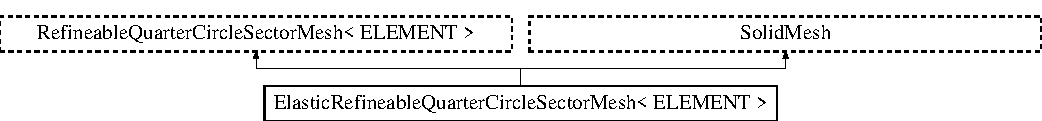
\includegraphics[height=1.623188cm]{classElasticRefineableQuarterCircleSectorMesh}
\end{center}
\end{figure}
\subsection*{Public Member Functions}
\begin{DoxyCompactItemize}
\item 
\hyperlink{classElasticRefineableQuarterCircleSectorMesh_a123699deecd2a908a7a882a9d2a9f4dd}{Elastic\+Refineable\+Quarter\+Circle\+Sector\+Mesh} (Geom\+Object $\ast$wall\+\_\+pt, const double \&xi\+\_\+lo, const double \&fract\+\_\+mid, const double \&xi\+\_\+hi, Time\+Stepper $\ast$time\+\_\+stepper\+\_\+pt=\&Mesh\+::\+Default\+\_\+\+Time\+Stepper)
\begin{DoxyCompactList}\small\item\em Constructor\+: Build mesh and copy Eulerian coords to Lagrangian ones so that the initial configuration is the stress-\/free one. \end{DoxyCompactList}\end{DoxyCompactItemize}


\subsection{Detailed Description}
\subsubsection*{template$<$class E\+L\+E\+M\+E\+NT$>$\newline
class Elastic\+Refineable\+Quarter\+Circle\+Sector\+Mesh$<$ E\+L\+E\+M\+E\+N\+T $>$}

Elastic quarter circle sector mesh\+: We \char`\"{}upgrade\char`\"{} the Refineable\+Quarter\+Circle\+Sector\+Mesh to become an Solid\+Mesh and equate the Eulerian and Lagrangian coordinates, thus making the domain represented by the mesh the stress-\/free configuration. 

Definition at line 363 of file disk\+\_\+oscillation.\+cc.



\subsection{Constructor \& Destructor Documentation}
\mbox{\Hypertarget{classElasticRefineableQuarterCircleSectorMesh_a123699deecd2a908a7a882a9d2a9f4dd}\label{classElasticRefineableQuarterCircleSectorMesh_a123699deecd2a908a7a882a9d2a9f4dd}} 
\index{Elastic\+Refineable\+Quarter\+Circle\+Sector\+Mesh@{Elastic\+Refineable\+Quarter\+Circle\+Sector\+Mesh}!Elastic\+Refineable\+Quarter\+Circle\+Sector\+Mesh@{Elastic\+Refineable\+Quarter\+Circle\+Sector\+Mesh}}
\index{Elastic\+Refineable\+Quarter\+Circle\+Sector\+Mesh@{Elastic\+Refineable\+Quarter\+Circle\+Sector\+Mesh}!Elastic\+Refineable\+Quarter\+Circle\+Sector\+Mesh@{Elastic\+Refineable\+Quarter\+Circle\+Sector\+Mesh}}
\subsubsection{\texorpdfstring{Elastic\+Refineable\+Quarter\+Circle\+Sector\+Mesh()}{ElasticRefineableQuarterCircleSectorMesh()}}
{\footnotesize\ttfamily template$<$class E\+L\+E\+M\+E\+NT$>$ \\
\hyperlink{classElasticRefineableQuarterCircleSectorMesh}{Elastic\+Refineable\+Quarter\+Circle\+Sector\+Mesh}$<$ E\+L\+E\+M\+E\+NT $>$\+::\hyperlink{classElasticRefineableQuarterCircleSectorMesh}{Elastic\+Refineable\+Quarter\+Circle\+Sector\+Mesh} (\begin{DoxyParamCaption}\item[{Geom\+Object $\ast$}]{wall\+\_\+pt,  }\item[{const double \&}]{xi\+\_\+lo,  }\item[{const double \&}]{fract\+\_\+mid,  }\item[{const double \&}]{xi\+\_\+hi,  }\item[{Time\+Stepper $\ast$}]{time\+\_\+stepper\+\_\+pt = {\ttfamily \&Mesh\+:\+:Default\+\_\+TimeStepper} }\end{DoxyParamCaption})\hspace{0.3cm}{\ttfamily [inline]}}



Constructor\+: Build mesh and copy Eulerian coords to Lagrangian ones so that the initial configuration is the stress-\/free one. 

Check that the element type is derived from the Solid\+Finite\+Element 

Definition at line 373 of file disk\+\_\+oscillation.\+cc.



The documentation for this class was generated from the following file\+:\begin{DoxyCompactItemize}
\item 
\hyperlink{disk__oscillation_8cc}{disk\+\_\+oscillation.\+cc}\end{DoxyCompactItemize}

\chapter{File Documentation}
\hypertarget{shock__disk_8cc}{}\section{shock\+\_\+disk.\+cc File Reference}
\label{shock__disk_8cc}\index{shock\+\_\+disk.\+cc@{shock\+\_\+disk.\+cc}}
\subsection*{Classes}
\begin{DoxyCompactItemize}
\item 
class \hyperlink{classElasticRefineableQuarterCircleSectorMesh}{Elastic\+Refineable\+Quarter\+Circle\+Sector\+Mesh$<$ E\+L\+E\+M\+E\+N\+T $>$}
\item 
class \hyperlink{classDiskShockWaveProblem}{Disk\+Shock\+Wave\+Problem$<$ E\+L\+E\+M\+E\+N\+T, T\+I\+M\+E\+S\+T\+E\+P\+P\+E\+R $>$}
\end{DoxyCompactItemize}
\subsection*{Namespaces}
\begin{DoxyCompactItemize}
\item 
 \hyperlink{namespaceGlobal__Physical__Variables}{Global\+\_\+\+Physical\+\_\+\+Variables}
\begin{DoxyCompactList}\small\item\em Global variables. \end{DoxyCompactList}\end{DoxyCompactItemize}
\subsection*{Functions}
\begin{DoxyCompactItemize}
\item 
void \hyperlink{namespaceGlobal__Physical__Variables_a19f4e20a92e7d216b4d2b00308f96917}{Global\+\_\+\+Physical\+\_\+\+Variables\+::constant\+\_\+pressure} (const Vector$<$ double $>$ \&xi, const Vector$<$ double $>$ \&x, const Vector$<$ double $>$ \&n, Vector$<$ double $>$ \&traction)
\begin{DoxyCompactList}\small\item\em Constant pressure load. \end{DoxyCompactList}\item 
int \hyperlink{shock__disk_8cc_a0ddf1224851353fc92bfbff6f499fa97}{main} (int argc, char $\ast$argv\mbox{[}$\,$\mbox{]})
\begin{DoxyCompactList}\small\item\em Driver for simple elastic problem. \end{DoxyCompactList}\end{DoxyCompactItemize}
\subsection*{Variables}
\begin{DoxyCompactItemize}
\item 
Constitutive\+Law $\ast$ \hyperlink{namespaceGlobal__Physical__Variables_a2a37fb040c832ee7a086bb13bb02a100}{Global\+\_\+\+Physical\+\_\+\+Variables\+::\+Constitutive\+\_\+law\+\_\+pt}
\begin{DoxyCompactList}\small\item\em Pointer to constitutive law. \end{DoxyCompactList}\item 
double \hyperlink{namespaceGlobal__Physical__Variables_a09a019474b7405b35da2437f7779bc7e}{Global\+\_\+\+Physical\+\_\+\+Variables\+::E} =1.\+0
\begin{DoxyCompactList}\small\item\em Elastic modulus. \end{DoxyCompactList}\item 
double \hyperlink{namespaceGlobal__Physical__Variables_a3962c36313826b19f216f6bbbdd6a477}{Global\+\_\+\+Physical\+\_\+\+Variables\+::\+Nu} =0.\+3
\begin{DoxyCompactList}\small\item\em Poisson\textquotesingle{}s ratio. \end{DoxyCompactList}\item 
double \hyperlink{namespaceGlobal__Physical__Variables_a23c2ade6398f54040b869f7f3a2bcc4b}{Global\+\_\+\+Physical\+\_\+\+Variables\+::P} = 0.\+00
\begin{DoxyCompactList}\small\item\em Uniform pressure. \end{DoxyCompactList}\end{DoxyCompactItemize}


\subsection{Function Documentation}
\mbox{\Hypertarget{shock__disk_8cc_a0ddf1224851353fc92bfbff6f499fa97}\label{shock__disk_8cc_a0ddf1224851353fc92bfbff6f499fa97}} 
\index{shock\+\_\+disk.\+cc@{shock\+\_\+disk.\+cc}!main@{main}}
\index{main@{main}!shock\+\_\+disk.\+cc@{shock\+\_\+disk.\+cc}}
\subsubsection{\texorpdfstring{main()}{main()}}
{\footnotesize\ttfamily int main (\begin{DoxyParamCaption}\item[{int}]{argc,  }\item[{char $\ast$}]{argv\mbox{[}$\,$\mbox{]} }\end{DoxyParamCaption})}



Driver for simple elastic problem. 



Definition at line 842 of file shock\+\_\+disk.\+cc.



References Global\+\_\+\+Physical\+\_\+\+Variables\+::\+Constitutive\+\_\+law\+\_\+pt, Global\+\_\+\+Physical\+\_\+\+Variables\+::E, Global\+\_\+\+Physical\+\_\+\+Variables\+::\+Nu, and Disk\+Shock\+Wave\+Problem$<$ E\+L\+E\+M\+E\+N\+T, T\+I\+M\+E\+S\+T\+E\+P\+P\+E\+R $>$\+::run().


\hypertarget{shock__disk_8txt__doxygenified_8h}{}\section{shock\+\_\+disk.\+txt\+\_\+doxygenified.\+h File Reference}
\label{shock__disk_8txt__doxygenified_8h}\index{shock\+\_\+disk.\+txt\+\_\+doxygenified.\+h@{shock\+\_\+disk.\+txt\+\_\+doxygenified.\+h}}

%--- End generated contents ---

% Index
\backmatter
\newpage
\phantomsection
\clearemptydoublepage
\addcontentsline{toc}{chapter}{Index}
\printindex

